\documentclass{amsart}
\usepackage{mathtools,upref,siunitx,upquote,fancyvrb,bbm,xspace,color}
\usepackage[hyphens]{url}
\usepackage[utf8]{inputenc}
\usepackage{esdiff}
\usepackage{graphicx}
\usepackage{xcolor}

\DeclareSymbolFont{GreekLetters}{OML}{cmr}{m}{it} %Provide missing letters
\DeclareSymbolFont{UpSfGreekLetters}{U}{cmss}{m}{n} %Provide missing letters
\DeclareMathSymbol{\varrho}{\mathalpha}{GreekLetters}{"25}
\DeclareMathSymbol{\UpSfLambda}{\mathalpha}{UpSfGreekLetters}{"03}
\DeclareMathSymbol{\UpSfSigma}{\mathalpha}{UpSfGreekLetters}{"06}
%\newcommand{\bvec}[1]{\boldsymbol{#1}}
\providecommand{\mathbold}{\boldsymbol}
\newcommand{\bvec}[1]{\mathbold{#1}}
%\newcommand{\bvec}[1]{\text{\boldmath$#1$}}
\newcommand{\avec}[1]{\vec{#1}}
%\renewcommand{\vec}[1] {\text{\boldmath$#1$}}
%\renewcommand{\vec}[1]{\ensuremath{\mathbf{#1}}}
%\newcommand{\vecsym}[1]{\ensuremath{\boldsymbol{#1}}}
\newcommand{\vecsym}[1]{\ensuremath{\mathbold{#1}}}
\def\bbl{\text{\boldmath$\{$}}
\def\bbr{\text{\boldmath$\}$}}
\newcommand{\bbrace}[1]{\bbl #1 \bbr}
\newcommand{\bbbrace}[1]{\mathopen{\pmb{\bigg\{}}#1\mathclose{\pmb{\bigg\}}}}
\def\betahat{\hat\beta}
\newcommand{\dif}{{\rm d}}

\newlength{\overwdth}
\def\overstrike#1{ 
\settowidth{\overwdth}{#1}\makebox[0pt][l]{\rule[0.5ex]{\overwdth}{0.1ex}}#1}

\makeatletter
\newcommand*\bigcdot{\mathpalette\bigcdot@{.7}}
\newcommand*\bigcdot@[2]{\mathbin{\vcenter{\hbox{\scalebox{#2}{$\m@th#1\bullet$}}}}}
\makeatother

\def\abs#1{\ensuremath{\left \lvert #1 \right \rvert}}
\newcommand{\normabs}[1]{\ensuremath{\lvert #1 \rvert}}
\newcommand{\bigabs}[1]{\ensuremath{\bigl \lvert #1 \bigr \rvert}}
\newcommand{\Bigabs}[1]{\ensuremath{\Bigl \lvert #1 \Bigr \rvert}}
\newcommand{\biggabs}[1]{\ensuremath{\biggl \lvert #1 \biggr \rvert}}
\newcommand{\Biggabs}[1]{\ensuremath{\Biggl \lvert #1 \Biggr \rvert}}
\newcommand{\norm}[2][{}]{\ensuremath{\left \lVert #2 \right \rVert}_{#1}}
\newcommand{\normnorm}[2][{}]{\ensuremath{\lVert #2 \rVert}_{#1}}
\newcommand{\bignorm}[2][{}]{\ensuremath{\bigl \lVert #2 \bigr \rVert}_{#1}}
\newcommand{\Bignorm}[2][{}]{\ensuremath{\Bigl \lVert #2 \Bigr \rVert}_{#1}}
\newcommand{\biggnorm}[2][{}]{\ensuremath{\biggl \lVert #2 \biggr \rVert}_{#1}}
\newcommand{\Biggnorm}[2][{}]{\ensuremath{\Biggl \lVert #2 \Biggr \rVert}_{#1}}
\newcommand{\ip}[3][{}]{\ensuremath{\left \langle #2, #3 \right \rangle_{#1}}}

\newcommand{\bigvecpar}[3]{\ensuremath{\bigl ( #1 \bigr )_{#2}^{#3}}}
\newcommand{\Bigvecpar}[3]{\ensuremath{\Bigl ( #1 \Bigr )_{#2}^{#3}}}
\newcommand{\biggvecpar}[3]{\ensuremath{\biggl ( #1 \biggr )_{#2}^{#3}}}
\newcommand{\bigpar}[1]{\ensuremath{\bigl ( #1 \bigr )}}
\newcommand{\Bigpar}[1]{\ensuremath{\Bigl ( #1 \Bigr )}}
\newcommand{\biggpar}[1]{\ensuremath{\biggl ( #1 \biggr )}}

\newcommand{\IIDsim}{\overset{\textup{IID}}{\sim}}
\newcommand{\LDsim}{\overset{\textup{LD}}{\sim}}

\DeclareMathOperator{\success}{succ}
\DeclareMathOperator{\sinc}{sinc}
\DeclareMathOperator{\sech}{sech}
\DeclareMathOperator{\csch}{csch}
\DeclareMathOperator{\dist}{dist}
\DeclareMathOperator{\spn}{span}
\DeclareMathOperator{\sgn}{sgn}
\DeclareMathOperator*{\rmse}{rmse}
\DeclareMathOperator{\Prob}{\mathbb{P}}
\DeclareMathOperator{\Ex}{\mathbb{E}}
\DeclareMathOperator{\rank}{rank}
\DeclareMathOperator{\erfc}{erfc}
\DeclareMathOperator{\erf}{erf}
\DeclareMathOperator{\cov}{cov}
\DeclareMathOperator{\cost}{cost}
\DeclareMathOperator{\comp}{comp}
\DeclareMathOperator{\corr}{corr}
\DeclareMathOperator{\diag}{diag}
\DeclareMathOperator{\var}{var}
\DeclareMathOperator{\opt}{opt}
\DeclareMathOperator{\brandnew}{new}
\DeclareMathOperator{\std}{std}
\DeclareMathOperator{\kurt}{kurt}
\DeclareMathOperator{\med}{med}
\DeclareMathOperator{\vol}{vol}
\DeclareMathOperator{\bias}{bias}
\DeclareMathOperator*{\argmax}{argmax}
\DeclareMathOperator*{\argmin}{argmin}
\DeclareMathOperator{\sign}{sign}
\DeclareMathOperator{\spann}{span}
\DeclareMathOperator{\cond}{cond}
\DeclareMathOperator{\trace}{trace}
\DeclareMathOperator{\Si}{Si}
%\DeclareMathOperator{\diag}{diag}
\DeclareMathOperator{\col}{col}
\DeclareMathOperator{\nullspace}{null}
\DeclareMathOperator{\Order}{{\mathcal O}}
%\DeclareMathOperator{\rank}{rank}

\newcommand{\vzero}{\bvec{0}}
\newcommand{\vone}{\bvec{1}}
\newcommand{\vinf}{\bvec{\infty}}
\newcommand{\va}{\bvec{a}}
\newcommand{\vA}{\bvec{A}}
\newcommand{\vb}{\bvec{b}}
\newcommand{\vB}{\bvec{B}}
\newcommand{\vc}{\bvec{c}}
\newcommand{\vC}{\bvec{C}}
\newcommand{\vd}{\bvec{d}}
\newcommand{\vD}{\bvec{D}}
\newcommand{\ve}{\bvec{e}}
\newcommand{\vf}{\bvec{f}}
\newcommand{\vF}{\bvec{F}}
\newcommand{\vg}{\bvec{g}}
\newcommand{\vG}{\bvec{G}}
\newcommand{\vh}{\bvec{h}}
\newcommand{\vi}{\bvec{i}}
\newcommand{\vj}{\bvec{j}}
\newcommand{\vk}{\bvec{k}}
\newcommand{\vK}{\bvec{K}}
\newcommand{\vl}{\bvec{l}}
\newcommand{\vell}{\bvec{\ell}}
\newcommand{\vL}{\bvec{L}}
\newcommand{\vm}{\bvec{m}}
\newcommand{\vp}{\bvec{p}}
\newcommand{\vq}{\bvec{q}}
\newcommand{\vr}{\bvec{r}}
\newcommand{\vs}{\bvec{s}}
\newcommand{\vS}{\bvec{S}}
\newcommand{\vt}{\bvec{t}}
\newcommand{\vT}{\bvec{T}}
\newcommand{\vu}{\bvec{u}}
\newcommand{\vU}{\bvec{U}}
\newcommand{\vv}{\bvec{v}}
\newcommand{\vV}{\bvec{V}}
\newcommand{\vw}{\bvec{w}}
\newcommand{\vW}{\bvec{W}}
\newcommand{\vx}{\bvec{x}}
\newcommand{\vX}{\bvec{X}}
\newcommand{\vy}{\bvec{y}}
\newcommand{\vY}{\bvec{Y}}
\newcommand{\vz}{\bvec{z}}
\newcommand{\vZ}{\bvec{Z}}

\newcommand{\ai}{\avec{\imath}}
\newcommand{\ak}{\avec{k}}
\newcommand{\avi}{\avec{\bvec{\imath}}}
\newcommand{\at}{\avec{t}}
\newcommand{\avt}{\avec{\vt}}
\newcommand{\ax}{\avec{x}}
\newcommand{\ah}{\avec{h}}
\newcommand{\akappa}{\avec{\kappa}}
\newcommand{\avx}{\avec{\vx}}
\newcommand{\ay}{\avec{y}}
\newcommand{\avy}{\avec{\vy}}
\newcommand{\avz}{\avec{\vz}}
\newcommand{\avzero}{\avec{\vzero}}
\newcommand{\aomega}{\avec{\omega}}
\newcommand{\avomega}{\avec{\vomega}}
\newcommand{\anu}{\avec{\nu}}
\newcommand{\avnu}{\avec{\vnu}}
\newcommand{\aDelta}{\avec{\Delta}}
\newcommand{\avDelta}{\avec{\vDelta}}

\newcommand{\valpha}{\bvec{\alpha}}
\newcommand{\vbeta}{\bvec{\beta}}
\newcommand{\vgamma}{\bvec{\gamma}}
\newcommand{\vGamma}{\bvec{\Gamma}}
\newcommand{\vdelta}{\bvec{\delta}}
\newcommand{\vDelta}{\bvec{\Delta}}
\newcommand{\vphi}{\bvec{\phi}}
\newcommand{\vvphi}{\bvec{\varphi}}
\newcommand{\vPhi}{\bvec{\Phi}}
\newcommand{\vomega}{\bvec{\omega}}
\newcommand{\vkappa}{\bvec{\kappa}}
\newcommand{\vlambda}{\bvec{\lambda}}
\newcommand{\vmu}{\bvec{\mu}}
\newcommand{\vnu}{\bvec{\nu}}
\newcommand{\vpsi}{\bvec{\psi}}
\newcommand{\vPsi}{\bvec{\Psi}}
\newcommand{\vepsilon}{\bvec{\epsilon}}
\newcommand{\veps}{\bvec{\varepsilon}}
\newcommand{\veta}{\bvec{\eta}}
\newcommand{\vxi}{\bvec{\xi}}
\newcommand{\vtheta}{\bvec{\theta}}
\newcommand{\vtau}{\bvec{\tau}}
\newcommand{\vzeta}{\bvec{\zeta}}

\newcommand{\hA}{\widehat{A}}
\newcommand{\hvb}{\hat{\vb}}
\newcommand{\hcc}{\widehat{\cc}}
\newcommand{\hD}{\widehat{D}}
\newcommand{\hE}{\widehat{E}}
\newcommand{\hf}{\widehat{f}}
\newcommand{\hF}{\widehat{F}}
\newcommand{\hg}{\hat{g}}
\newcommand{\hvf}{\widehat{\bvec{f}}}
\newcommand{\hh}{\hat{h}}
\newcommand{\hH}{\widehat{H}}
\newcommand{\hi}{\hat{\imath}}
\newcommand{\hI}{\hat{I}}
\newcommand{\hci}{\widehat{\ci}}
\newcommand{\hj}{\hat{\jmath}}
\newcommand{\hJ}{\widehat{J}}
\newcommand{\hp}{\hat{p}}
\newcommand{\hP}{\widehat{P}}
\newcommand{\hS}{\widehat{S}}
\newcommand{\hv}{\hat{v}}
\newcommand{\hV}{\widehat{V}}
\newcommand{\hx}{\hat{x}}
\newcommand{\hX}{\widehat{X}}
\newcommand{\hvX}{\widehat{\vX}}
\newcommand{\hy}{\hat{y}}
\newcommand{\hvy}{\hat{\vy}}
\newcommand{\hY}{\widehat{Y}}
\newcommand{\hvY}{\widehat{\vY}}
\newcommand{\hZ}{\widehat{Z}}
\newcommand{\hvZ}{\widehat{\vZ}}

\newcommand{\halpha}{\hat{\alpha}}
\newcommand{\hvalpha}{\hat{\valpha}}
\newcommand{\hbeta}{\hat{\beta}}
\newcommand{\hvbeta}{\hat{\vbeta}}
\newcommand{\hgamma}{\hat{\gamma}}
\newcommand{\hvgamma}{\hat{\vgamma}}
\newcommand{\hdelta}{\hat{\delta}}
\newcommand{\hvareps}{\hat{\varepsilon}}
\newcommand{\hveps}{\hat{\veps}}
\newcommand{\hmu}{\hat{\mu}}
\newcommand{\hnu}{\hat{\nu}}
\newcommand{\hvnu}{\widehat{\vnu}}
\newcommand{\homega}{\widehat{\omega}}
\newcommand{\hPi}{\widehat{\Pi}}
\newcommand{\hrho}{\hat{\rho}}
\newcommand{\hsigma}{\hat{\sigma}}
\newcommand{\htheta}{\hat{\theta}}
\newcommand{\hTheta}{\hat{\Theta}}
\newcommand{\htau}{\hat{\tau}}
\newcommand{\hxi}{\hat{\xi}}
\newcommand{\hvxi}{\hat{\vxi}}

\newcommand{\otau}{\overline{\tau}}
\newcommand{\oY}{\overline{Y}}

\newcommand{\rD}{\mathring{D}}
\newcommand{\rf}{\mathring{f}}
\newcommand{\rV}{\mathring{V}}

\newcommand{\ta}{\tilde{a}}
\newcommand{\tA}{\tilde{A}}
\newcommand{\tmA}{\widetilde{\mA}}
\newcommand{\tvb}{\widetilde{\vb}}
\newcommand{\tcb}{\widetilde{\cb}}
\newcommand{\tB}{\widetilde{B}}
\newcommand{\tc}{\tilde{c}}
\newcommand{\tvc}{\tilde{\vc}}
\newcommand{\tfc}{\tilde{\fc}}
\newcommand{\tC}{\widetilde{C}}
\newcommand{\tcc}{\widetilde{\cc}}
\newcommand{\tD}{\widetilde{D}}
\newcommand{\te}{\tilde{e}}
\newcommand{\tE}{\widetilde{E}}
\newcommand{\tf}{\widetilde{f}}
\newcommand{\tF}{\widetilde{F}}
\newcommand{\tvf}{\tilde{\vf}}
\newcommand{\tcf}{\widetilde{\cf}}
\newcommand{\tg}{\tilde{g}}
\newcommand{\tvg}{\widetilde{\vg}}
\newcommand{\tG}{\widetilde{G}}
\newcommand{\tildeh}{\tilde{h}}
\newcommand{\tH}{\widetilde{H}}
\newcommand{\tch}{\widetilde{\ch}}
\newcommand{\tK}{\widetilde{K}}
\newcommand{\tvk}{\tilde{\vk}}
\newcommand{\tM}{\widetilde{M}}
\newcommand{\tn}{\tilde{n}}
\newcommand{\tN}{\widetilde{N}}
\newcommand{\tQ}{\widetilde{Q}}
\newcommand{\tR}{\widetilde{R}}
\newcommand{\tS}{\widetilde{S}}
\newcommand{\tvS}{\widetilde{\vS}}
\newcommand{\tT}{\widetilde{T}}
\newcommand{\tv}{\tilde{v}}
\newcommand{\tV}{\widetilde{V}}
\newcommand{\tvx}{\tilde{\vx}}
\newcommand{\tW}{\widetilde{W}}
\newcommand{\tx}{\tilde{x}}
\newcommand{\tX}{\widetilde{X}}
\newcommand{\tvX}{\widetilde{\vX}}
\newcommand{\ty}{\tilde{y}}
\newcommand{\tvy}{\tilde{\vy}}
\newcommand{\tz}{\tilde{z}}
\newcommand{\tZ}{\widetilde{Z}}
\newcommand{\tL}{\widetilde{L}}
\newcommand{\tP}{\widetilde{P}}
\newcommand{\tY}{\widetilde{Y}}
\newcommand{\tmH}{\widetilde{\mH}}
\newcommand{\tmK}{\widetilde{\mK}}
\newcommand{\tmM}{\widetilde{\mM}}
\newcommand{\tmQ}{\widetilde{\mQ}}
\newcommand{\tct}{\widetilde{\ct}}
\newcommand{\talpha}{\tilde{\alpha}}
\newcommand{\tdelta}{\tilde{\delta}}
\newcommand{\tDelta}{\tilde{\Delta}}
\newcommand{\tvareps}{\tilde{\varepsilon}}
\newcommand{\tveps}{\tilde{\veps}}
\newcommand{\tlambda}{\tilde{\lambda}}
\newcommand{\tmu}{\tilde{\mu}}
\newcommand{\tnu}{\tilde{\nu}}
\newcommand{\trho}{\tilde{\rho}}
\newcommand{\tvarrho}{\tilde{\varrho}}
\newcommand{\ttheta}{\tilde{\theta}}
\newcommand{\tsigma}{\tilde{\sigma}}
\newcommand{\tvmu}{\tilde{\vmu}}
\newcommand{\tphi}{\tilde{\phi}}
\newcommand{\tPhi}{\widetilde{\Phi}}
\newcommand{\tvphi}{\tilde{\vphi}}
\newcommand{\ttau}{\tilde{\tau}}
\newcommand{\txi}{\tilde{\xi}}
\newcommand{\tvxi}{\tilde{\vxi}}


\newcommand{\mA}{\mathsf{A}}
\newcommand{\mB}{\mathsf{B}}
\newcommand{\mC}{\mathsf{C}}
\newcommand{\vmC}{\bvec{\mC}}
\newcommand{\mD}{\mathsf{D}}
\newcommand{\mF}{\mathsf{F}}
\newcommand{\mG}{\mathsf{G}}
\newcommand{\mH}{\mathsf{H}}
\newcommand{\mI}{\mathsf{I}}
\newcommand{\mK}{\mathsf{K}}
\newcommand{\mL}{\mathsf{L}}
\newcommand{\mM}{\mathsf{M}}
\newcommand{\mP}{\mathsf{P}}
\newcommand{\mQ}{\mathsf{Q}}
\newcommand{\mR}{\mathsf{R}}
\newcommand{\mS}{\mathsf{S}}
\newcommand{\mT}{\mathsf{T}}
\newcommand{\mU}{\mathsf{U}}
\newcommand{\mV}{\mathsf{V}}
\newcommand{\mW}{\mathsf{W}}
\newcommand{\mX}{\mathsf{X}}
\newcommand{\mLambda}{\UpSfLambda}
\newcommand{\mSigma}{\UpSfSigma}
\newcommand{\mzero}{\mathsf{0}}
\newcommand{\mGamma}{\mathsf{\Gamma}}

\newcommand{\bbE}{\mathbb{E}}
\newcommand{\bbF}{\mathbb{F}}
\newcommand{\bbK}{\mathbb{K}}
\newcommand{\bbV}{\mathbb{V}}
\newcommand{\bbZ}{\mathbb{Z}}
\newcommand{\bbone}{\mathbbm{1}}
\newcommand{\naturals}{\mathbb{N}}
\newcommand{\reals}{\mathbb{R}}
\newcommand{\integers}{\mathbb{Z}}
\newcommand{\natzero}{\mathbb{N}_{0}}
\newcommand{\rationals}{\mathbb{Q}}
\newcommand{\complex}{\mathbb{C}}

\newcommand{\ca}{\mathcal{A}}
\newcommand{\cb}{\mathcal{B}}
\providecommand{\cc}{\mathcal{C}}
\newcommand{\cd}{\mathcal{D}}
\newcommand{\ce}{\mathcal{E}}
\newcommand{\cf}{\mathcal{F}}
\newcommand{\cg}{\mathcal{G}}
\newcommand{\ch}{\mathcal{H}}
\newcommand{\ci}{\mathcal{I}}
\newcommand{\cj}{\mathcal{J}}
\newcommand{\ck}{\mathcal{K}}
\newcommand{\cl}{\mathcal{L}}
\newcommand{\cm}{\mathcal{M}}
\newcommand{\tcm}{\widetilde{\cm}}
\newcommand{\cn}{\mathcal{N}}
\newcommand{\cp}{\mathcal{P}}
\newcommand{\calr}{\mathcal{R}}
\newcommand{\cs}{\mathcal{S}}
\newcommand{\ct}{\mathcal{T}}
\newcommand{\cu}{\mathcal{U}}
\newcommand{\cv}{\mathcal{V}}
\newcommand{\cw}{\mathcal{W}}
\newcommand{\cx}{\mathcal{X}}
\newcommand{\tcx}{\widetilde{\cx}}
\newcommand{\cy}{\mathcal{Y}}
\newcommand{\cz}{\mathcal{Z}}

\newcommand{\fc}{\mathfrak{c}}
\newcommand{\fC}{\mathfrak{C}}
\newcommand{\fh}{\mathfrak{h}}
\newcommand{\fu}{\mathfrak{u}}

\newcommand{\me}{\ensuremath{\mathrm{e}}} % for math number 'e', 2.718 281 8..., tha base of natural logarithms
\newcommand{\mi}{\ensuremath{\mathrm{i}}} % for math number 'i', the imaginary unit
\newcommand{\mpi}{\ensuremath{\mathrm{\pi}}} % for math number 'pi', the circumference of a circle of diameter 1



\usepackage{algpseudocode}
\usepackage{algorithm, algorithmicx}
\algnewcommand\algorithmicparam{\textbf{Parameters:}}
\algnewcommand\PARAM{\item[\algorithmicparam]}
\algnewcommand\algorithmicinput{\textbf{Input:}}
\algnewcommand\INPUT{\item[\algorithmicinput]}
\algnewcommand\RETURN{\State \textbf{Return }}

\newcommand{\tr}{\widetilde{r}}
\newcommand{\appxintn}{\appxint_n}
\DeclareMathOperator{\appxint}{\hat{I}}
\DeclareMathOperator{\trun}{trunc}

\newcommand{\FredNote}[1]{{\color{blue}#1}}

\newcommand{\LarysaNote}[1]{{\color{violet}#1}}



\begin{document}
\title{The Quality of Lattice Sequences}
\author{Larysa Matiukha}
\author{Yuhan Ding}
\author{Fred J. Hickernell}
\begin{abstract}This project is where all of the files and commands go that are needed elsewhere
\end{abstract}

\maketitle

\begin{itemize}
    \item finish the derivation for $n = \lambda 2^p$ and add log terms 
    \item derive the bounds on other figures of merit
    \item replace base 2 by arbitrary prime base (b)
    \item add more explanation, motivation 
    \item derive bound for arbitrary $s$ and $\gamma$
    \item derive the bounds for $Q_{2\alpha}$
\end{itemize}

\section{Introduction}
Lattices are a popular choice of nodes $\{\vz_i\}_{i=0}^{n-1} \in [0,1)^s$ for approximating multidimensional integrals by a sample mean,
\[
\int_{[0,1)^s} f(\vx) \, \dif \vx \approx \frac{1}{n} \sum_{i=0}^{n-1} f(\vz_i) =:\appxint(f),
\]
\cite{DicEtal22a,Nie92,SloJoe94}.
Historically, lattice points were initially constructed as sets with fixed cardinality, $n$, and took the form
\begin{equation} \label{eq:lat}
    \{\vz_i = i \vh/n \pmod{\vone} : i=0,1, \ldots, n-1 \} \in [0,1)^s,
\end{equation}
where $\vh \in \{1, \ldots, n-1\}^s$ is the \emph{generating vector}.  A (random) shift, $\vDelta \in [0,1)^s$, is often added:
\begin{equation} \label{eq:shlat}
    \{\vz_i = i \vh/n + \vDelta \pmod{\vone} : i=0,1, \ldots, n-1 \} \in [0,1)^s.
\end{equation}

\begin{figure}[h]
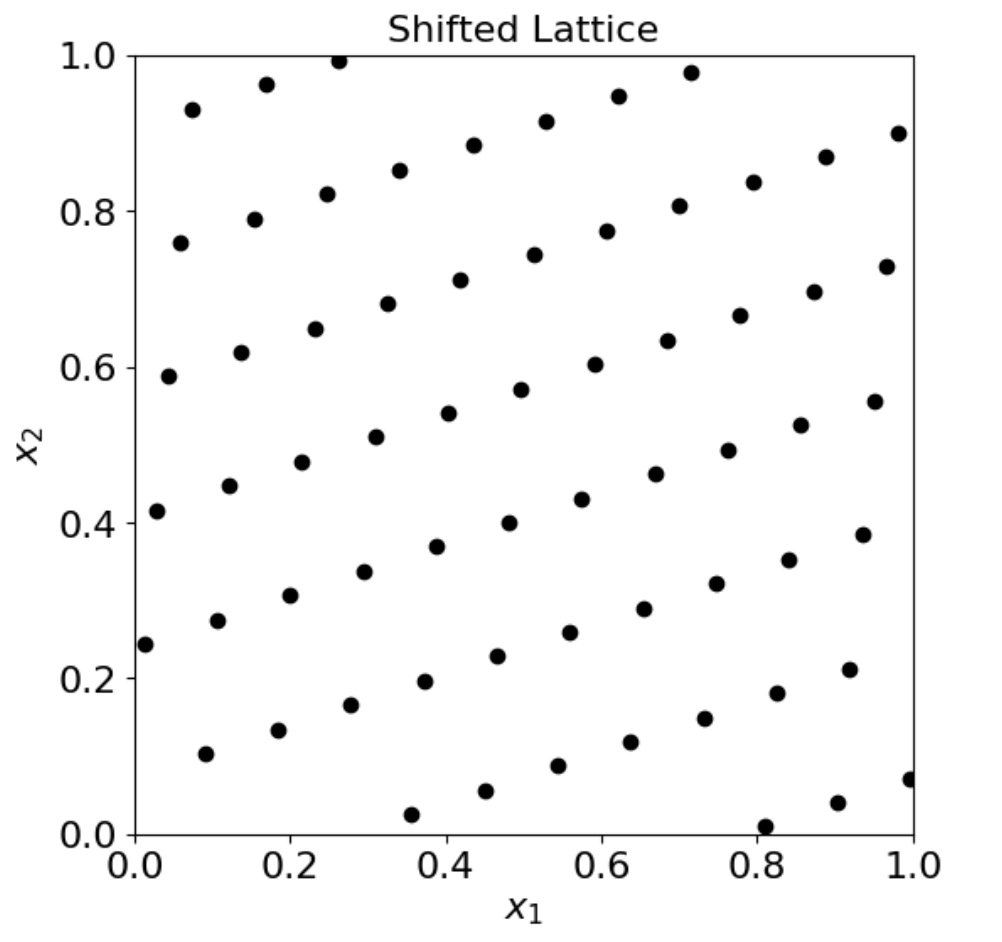
\includegraphics[width=5cm,trim={0 0 0 7.5mm},clip]{shifted-lattice}
\caption{Two-dimensional Shifted Lattice}
\label{fig:enter-label}
\end{figure}



Extensible lattice sequences were proposed by \cite{HicEtal00,Mai81a} and take the form
\begin{equation} \label{eq:extlat}
    \{\vz_i = \vh\phi(i)+ \vDelta \pmod{\vone} : i=0,1, \ldots \} \in [0,1)^s.
\end{equation}
where $\{\phi(\cdot)\}_{i=0}^\infty$ is the van der Corput sequence (in base 2 for now).  In this case $\vh$ must be a generalized integer as defined in \cite[Section 2]{HicNie03a}.

For the van der Corput sequence
\[
\phi((\cdots i_2 i_1 i_0)_2) = {}_20.i_0 i_1 i_2 \cdots.
\]
For example,
\[
\phi(6) = \phi(110_2) = {}_20.011 = \frac 38.
\]
Note that
\begin{equation} \label{eq:phipropone}
\{ \phi(i) : i = 0, \ldots, b^m-1 \} = \{0, b^{-m}, 2\times b^{-m}, \ldots, 1 - b^{-m} \}.
\end{equation}
Also note that
\begin{multline} \label{eq:phiproptwo}
\{ \phi(i) : i = \lambda \times b^m , \ldots, (\lambda+1)b^m-1 \} \\
= \{\phi(\lambda \times b^m) + 0, \phi(\lambda \times b^m) + b^{-m}, \ldots, \phi(\lambda \times b^m) + 1 - b^{-m} \} , \\
\lambda \in \natzero.
\end{multline}


Hickernell and Niederreiter \cite{HicNie03a} established the existence of extensible lattices with good generating vectors for the preferred values $n = 2, 4, 8, \ldots$.  The purpose here is to extend these results to all $n>1$, recognizing that the upper bounds on the figures of merit will be somewhat worse.

We will fix $s$ and ignore $\vgamma$ for now.

\subsection{Worst case error analysis}
We first consider integrands, $f$, that have an absolutely summable Fourier series:
\begin{equation} \label{eq:fseries}
    f(\vx) = \sum_{\vk \in \integers^{s}} \tf(\vk) \me^{2 \pi \sqrt{-1} \vk^T \vx}, \qquad \tf(\vk) = \int_{[0,1)^{\infty}} f(\vx) \me^{-2 \pi \sqrt{-1} \vk^T \vx}\, \dif \vx
\end{equation}
Define the weights
\begin{equation}
\tr(\vk) = \prod_{j=1}^{s} r(k_{j},\gamma_{j}),
\qquad \text{where} \qquad r(k_{j},\gamma_{j})=\begin{cases} 1, &
k_{j}=0, \\ \gamma_{j}^{-1}\abs{k_{j}}, & k_{j} \ne 0.  \end{cases}
\end{equation}
Define a Banach
space of functions:
$$
\cf_{\alpha} = \{ f \in \cl_2[0,1)^{s} :
\norm[\cf{\alpha}]{f} < \infty \}, \qquad
\norm[\cf{\alpha}]{f} := \sup_{\vk \in \integers^{s}}
\left(\tr(\vk,\vgamma)^{\alpha} \abs{\tilde{f}(\vk)} \right).
$$



It then follows that the error in approximating the integral by the sample mean is
\begin{align} \label{eq:wcerrPalpha}
\abs{\int_{[0,1)^{s}} f(\vx) \, \dif \vx - \appxint_n(f)} &
= \abs{\sum_{\vk \in \integers^{s}} \tf(\vk) \left[\int_{[0,1)^{s}} \me^{2 \pi \sqrt{-1} \vk^T \vx} \, \dif \vx - \appxintn(\me^{2 \pi \sqrt{-1} \vk^T \cdot})\right]} \\
\nonumber
& = \abs{\sum_{\vk \in \integers^s \setminus\{\vzero\}} \tf(\vk) \left[ \appxintn(\me^{2 \pi \sqrt{-1} \vk^T \cdot})\right]} \\
\nonumber
& \le \norm[\cf{\alpha}]{f} \underbrace{\sum_{\vk \in \integers^s \setminus\{\vzero\}} \abs{\appxint_n(\me^{2 \pi \sqrt{-1} \vk^T \cdot})}\tr(\vk)^{-\alpha}}_{=: P_\alpha(\vh,\vgamma,n,1:s) = \text{quality of the lattice nodes}}  %\qquad \forall f \in \cf_{\alpha} \\
\nonumber
\end{align}

For $n = b^m$, the quality measure $P_\alpha(\vh,\vgamma,n,1:s)$ takes on a simple form.  Note that
\begin{align}\label{Eq:DualLattice}
    \MoveEqLeft{\appxint_{b^m}(\me^{2 \pi \sqrt{-1} \vk^T \cdot})} \\
    \nonumber
    &= \frac 1{b^m} \sum_{i=0}^{b^m-1} \me^{2 \pi \sqrt{-1} \vk^T (\vh\phi(i) + \vDelta \pmod{\vone})} \\
    \nonumber
    &= \frac {\me^{2 \pi \sqrt{-1} \vk^T \vDelta}}{b^m} \sum_{i=0}^{b^m-1} \me^{2 \pi \sqrt{-1} \vk^T \vh\phi(i)} \\
    \nonumber
    &= \frac {\me^{2 \pi \sqrt{-1} \vk^T \vDelta}}{b^m} \sum_{i=0}^{b^m-1} \me^{2 \pi \sqrt{-1} \vk^T \vh i/b^m} \qquad \text{by \eqref{eq:phipropone}}\\
    \nonumber
    &= \frac {\me^{2 \pi \sqrt{-1} \vk^T \vDelta}}{b^m} \times
    \begin{cases}
    \frac{\me^{2 \pi \sqrt{-1} \vk^T \vh} - 1}{\me^{2 \pi \sqrt{-1} \vk^T \vh/b^m} - 1} = 0, & \vk^T \vh \pmod{b^m} \ne 0\\
    b^m, & \vk^T \vh \pmod{b^m} = 0
    \end{cases} \\
    \nonumber
    & = \me^{2 \pi \sqrt{-1} \vk^T \vDelta} \bbone_{B(\vh,m,1:s)}(\vk)
\end{align}
Thus it follows that
\begin{equation} \label{eq:Palphadual}
    P_\alpha(\vh,\vgamma,b^m,1:s) = \sum_{\vk \in B(\vh,m,1:s)} \tr(\vk,\vgamma)^{-\alpha},
\end{equation}
where $B(\vh,m,1:s) : = \{\vk \in  \integers^s \setminus \{\vzero\} : \vk^T \vh \pmod{b^m} = 0\}$ is called the \emph{dual lattice}.  This corresponds to \cite[Equation (3)]{HicNie03a}, and we know by \cite[Theorem 5]{HicNie03a} that  there exists $\vh$ with
\begin{multline} \label{eq:Niedbd}
    P_{\alpha}(\vh,\vgamma,b^m,1:s) \le C_{R}(\alpha,\vgamma,\epsilon,s)
    b^{-m\alpha} \log(b^{m\alpha(s+1)}) [\log \log (
    b^m+1)]^{\alpha(1+\epsilon)}, \\ m = 1, 2,\ldots, \quad \alpha \ge 1.
\end{multline}

Note that
\begin{align*}
    P_{\alpha}(\vh,\vgamma,1,1:s) & = \sum_{\vk \ne \vzero} \tr(\vk, \vgamma)^{-\alpha} = -1 + \sum_{\vk \in \integers^s} \tr(\vk,\vgamma)^{-\alpha} \\
    & = -1 + \sum_{k_1 =-\infty}^{\infty} \cdots \sum_{k_s  =-\infty}^{\infty} \frac{1}{\prod_{j=1}^s[\max(1,\gamma_j^{-1}\abs{k_j})]^\alpha} \\
    & = -1 + \sum_{k_1 =-\infty}^{\infty} \frac{1}{[\max(1,\gamma_1^{-1}\abs{k_1})]^\alpha} \cdots \sum_{k_s  =-\infty}^{\infty} \frac{1}{[\max(1,\gamma_s^{-1}\abs{k_s})]^\alpha} \\
    & = -1 + \left[\sum_{k =-\infty}^{\infty} \frac{1}{[\max(1,\gamma^{-1}\abs{k})]^\alpha} \right]^d \\
    & = -1 + \left[1 + 2 \gamma^{\alpha} \sum_{k =1}^{\infty} \frac{1}{k^\alpha} \right]^d \\
    & = -1 + \left[1 + 2 \gamma^{\alpha}\zeta(\alpha) \right]^d
\end{align*}

Therefore, the above formula \eqref{eq:Niedbd} can be extended to the case of $m=0$:

\begin{multline} \label{eq:Palphaextm}
    P_{\alpha}(\vh,\vgamma,b^m,1:s) \\
    \le C_{R}(\alpha,\vgamma,\epsilon,s)
    b^{-m\alpha}\max(1, \log(b^{m\alpha(s+1)})) [\max(1,\log \log (
    b^m+1))]^{\alpha(1+\epsilon)}, \\ m =0, 1, 2,\ldots, \quad \alpha \ge 1.
\end{multline}


\subsection{Randomized Error Analysis}
Another approach is to assume that $f$ in \eqref{eq:fseries} is a random function (stochastic process) where
\begin{equation}
    \abs{\tf(\vk)} \IIDsim \cn(0,\tr(\vk)^{-2\alpha}).
\end{equation}
Then it follows that
\begin{align*}
    \MoveEqLeft{\Ex_f\left[\left(\int_{[0,1)^d} f(\vx) \, \dif \vx - \appxintn(f) \right)^2\right]} \\
    & =
    \Ex_f\left[\left(\sum_{\vk \in \integers^s \setminus\{\vzero\}} \tf(\vk) \appxintn(\me^{2 \pi \sqrt{-1} \vk^T \cdot})\right)^2\right] \\
     & =
    \Ex_f\left[\sum_{\vk,\vl \in \integers^s \setminus\{\vzero\}} \tf(\vk) \tf^*(\vl) \appxintn(\me^{2 \pi \sqrt{-1} \vk^T \cdot}) \appxintn(\me^{-2 \pi \sqrt{-1} \vl^T \cdot})\right] \\
    & = \underbrace{\sum_{\vk\in \integers^s \setminus\{\vzero\}} \tr(\vk)^{-2\alpha} \abs{\appxintn(\me^{2 \pi \sqrt{-1} \vk^T \cdot})}^2}_{Q_{2\alpha}(\vh,n) = \text{another measure of quality of the lattice nodes}}  \\
\end{align*}

\textbf{Research Question}  May we extend this result to all $n$ with perhaps some extra $\log(n)$ terms?

E.g.,  $n =6 = 0\cdot 1 + 1 \cdot 2 + 1 \cdot 4$, $m = 2$ $\vDelta = \vzero$.

\begin{align*}
   \MoveEqLeft{\appxint_{6}(\me^{2 \pi \sqrt{-1} \vk^T \cdot})}\\
    &= \frac 1{6} \sum_{i=0}^{5} \me^{2 \pi \sqrt{-1} \vk^T \vh\phi(i)} \\
    &= \frac {1}{6} \left\{ \sum_{i=0}^3 \me^{2 \pi \sqrt{-1} \vk^T \vh\phi(i)} + \sum_{i=4}^5 \me^{2 \pi \sqrt{-1} \vk^T \vh\phi(i)} + \sum_{i=6}^5 \me^{2 \pi \sqrt{-1} \vk^T \vh\phi(i)}  \right\} \\
    &= \frac {1}{6} \left\{ \sum_{i=0}^3 \me^{2 \pi \sqrt{-1} \vk^T \vh\phi(i)} + \sum_{i=0}^1 \me^{2 \pi \sqrt{-1} \vk^T \vh[\phi(i)+\phi(4)]} + \sum_{i=0}^{-1} \me^{2 \pi \sqrt{-1} \vk^T \vh[\phi(i)+\vphi(6)]}  \right\} \ \ \text{by \eqref{eq:phiproptwo}} \\
    &= \frac {1}{6} \left\{ 1\cdot\sum_{i=0}^{3}\me^{2 \pi \sqrt{-1} \vk^T \vh\phi(i)} + 1 \cdot \me^{2 \pi \sqrt{-1} \vk^T \phi(4)} \cdot \sum_{i=0}^{1}\me^{2 \pi \sqrt{-1} \vk^T \vh\phi(i)} \right . \\
    & \qquad \qquad \left . +  0 \cdot
    \me^{2 \pi \sqrt{-1} \vk^T \vh\phi(6)} \cdot \sum_{i=0}^{0}\me^{2 \pi \sqrt{-1} \vk^T \vh\phi(i)} \right\}
\end{align*}

 Then,
\begin{align*}
    P_\alpha(\vh,6) & = \sum_{\vk \in \integers^s \setminus\{\vzero\}}
    \abs{\appxint_6(\me^{2 \pi \sqrt{-1} \vk^T \cdot})}\tr(\vk)^{-\alpha}
    \\
    & \le
    \frac {1}{6} \left\{ 1\cdot\sum_{\vk \in \integers^s \setminus\{\vzero\}} \abs{\sum_{i=0}^{3}\me^{2 \pi \sqrt{-1} \vk^T \vh\phi(i)}} \tr(\vk)^{-\alpha}  \right .
    \\
    & \qquad \qquad + 1  \cdot \sum_{\vk \in \integers^s \setminus\{\vzero\}} \abs{\sum_{i=0}^{1}\me^{2 \pi \sqrt{-1} \vk^T \vh\phi(i)}} \tr(\vk)^{-\alpha}  \\
    & \qquad \qquad \left . +  0
    \cdot \sum_{\vk \in \integers^s \setminus\{\vzero\}} \abs{\sum_{i=0}^{0}\me^{2 \pi \sqrt{-1} \vk^T \vh\phi(i)}}  \tr(\vk)^{-\alpha} \right\}\\
    & =
    \frac {1}{6} \left\{ 1\cdot\sum_{\vk \in \integers^s \setminus\{\vzero\}} 4 \cdot \bbone_{B(\vh,2)}(\vk) \tr(\vk)^{-\alpha}  \right .
    + 1  \cdot \sum_{\vk \in \integers^s \setminus\{\vzero\}}2 \cdot \bbone_{B(\vh,1)}(\vk) \tr(\vk)^{-\alpha}  \\
    & \qquad \qquad \left . +  0
    \cdot \sum_{\vk \in \integers^s \setminus\{\vzero\}} 1 \cdot \bbone_{B(\vh,1)}(\vk)  \tr(\vk)^{-\alpha} \right\} \qquad \text{by \eqref{Eq:DualLattice}}\\
    & = \frac {1}{6} \left\{ 4 \cdot 1 \cdot P_\alpha(\vh,4)+ 2 \cdot 1 \cdot P_\alpha(\vh,2)+ 1 \cdot 0 \cdot P_\alpha(\vh,1) \right\} \\
\end{align*}

We know that and $P_\alpha(\vh,2^2) \le C_{R}(\alpha,\epsilon,s)
    2^{-2\alpha}$ and $P_\alpha(\vh,2^1) \le C_{R}(\alpha,\epsilon,s)
    2^{-\alpha} $. Then,
    \begin{align*}
        P_\alpha(\vh,6) & \le \frac {1}{6} \left\{ 4 \cdot 1 \cdot P_\alpha(\vh,4) + 2 \cdot 1 \cdot P_\alpha(\vh,2) \right\} \\
         & \le \frac {1}{6} \left\{C_{R}(\alpha,\epsilon,s)
         2^{2-2\alpha} + C_{R}(\alpha,\epsilon,s)
         2^{1-\alpha} \right\}
    \end{align*}


For any non-negative integer $n$, express as  $n = n_0 + bn_1 + \cdots + b^m n_m$, where the digits $n_0, n_1, \ldots$ are in $\{0, 1, \cdots, b-1\}$ .  Thus, $m = \lfloor \log_b(n) \rfloor$.  Let $\trun(n,\ell) = n_0 + \cdots + b^{\ell} n_{\ell}$ for $\ell = 0, \ldots, m$ and $\trun(n,-1) = 0$, then

\begin{align*}
    \MoveEqLeft{\appxint_{n}(\me^{2 \pi \sqrt{-1} \vk^T \cdot}) } \\
    &= \frac 1{n} \sum_{i=0}^{n-1} \me^{2 \pi \sqrt{-1} \vk^T (\vh\phi(i) + \vDelta \pmod{\vone})} \\
    \nonumber
    &= \frac {\me^{2 \pi \sqrt{-1} \vk^T \vDelta}}{n} \sum_{\ell = 0}^{m} \,
    \sum_{i=n - \trun(n,m-\ell) }^{n - \trun(n,m-\ell-1)  -1} \me^{2 \pi \sqrt{-1} \vk^T \vh\phi(i)} \\
    &= \frac {\me^{2 \pi \sqrt{-1} \vk^T \vDelta}}{n} \sum_{\ell = 0}^{m} \, n_{m-\ell}
    \sum_{i=0 }^{b^{m-\ell}  -1} \me^{2 \pi \sqrt{-1} \vk^T \vh[i/b^m + \phi(n - \trun(n,m-\ell))]} \\
    & \hspace{30ex} \text{by \eqref{eq:phiproptwo}} \\
    & = \frac {\me^{2 \pi \sqrt{-1} \vk^T \vDelta}}{n} \sum_{\ell = 0}^{m} b^{m-\ell} n_\ell \bbone_{B(\vh,m-\ell)}(\vk) \me^{2 \pi \sqrt{-1} \vk^T \vh\phi(n - \trun(n,m-\ell))}.
\end{align*}
This implies that
\begin{equation} \label{eq:ihatarbn}
    \abs{\appxint_{n}(\me^{2 \pi \sqrt{-1} \vk^T \cdot})} \le \frac {1}{n} \sum_{\ell = 0}^{m} b^{m-\ell} n_\ell \bbone_{B(\vh,m-\ell)}(\vk)
\end{equation}

Next we compute $P_\alpha(\vh,\vgamma,n,1:s)$ for this arbitrary $n$:
\begin{align*}
      P_\alpha(\vh,\vgamma,n,1:s) & = \sum_{\vk \in \integers^s \setminus\{\vzero\}} \abs{\appxint_n(\me^{2 \pi \sqrt{-1} \vk^T \cdot})}\tr(\vk)^{-\alpha} \qquad \text{by \eqref{eq:wcerrPalpha}} \\
      & \le \frac {1}{n} \sum_{\ell = 0}^{m} b^{m-\ell} n_{m - \ell} \sum_{\vk \in B(\vh,m-\ell,u)} \tr(\vk)^{-\alpha}
      \qquad \text{by \eqref{eq:ihatarbn}}\\
      & = \frac {1}{n} \sum_{\ell = 0}^{m} b^{m-\ell} n_{m - \ell} P_\alpha(\vh,\vgamma,b^{m-\ell},1:s)
      \qquad \text{by \eqref{eq:Palphadual}}\\
      & =  \frac {1}{n} \left\{ b^m n_m P_\alpha(\vh,\vgamma,b^m,1:s) + b^{m-1} n_{m-1} P_\alpha(\vh,\vgamma,b^{m-1},1:s) + \cdots + b^0 n_0 P_\alpha(\vh,\vgamma,b^0,1:s)  \right\} \\
      &\le \frac {(b-1)}{n} \left\{ b^m  P_\alpha(\vh,\vgamma,b^m,1:s) + b^{m-1}  P_\alpha(\vh,\vgamma,b^{m-1},1:s) + \cdots + 2^0  P_\alpha(\vh,\vgamma,b^0,1:s)  \right\} \\
      & \le \frac {(b-1)C_{R}(\alpha,\vgamma,\epsilon,s)}{n} \left\{ b^{m(1-\alpha)}\max(1, \log(b^{m\alpha(s+1)})) [\max(1,\log \log (
    b^m+1))]^{\alpha(1+\epsilon)}\right .\\ 
      & \qquad  + b^{(m-1)(1-\alpha)}\max(1, \log(b^{(m-1)\alpha(s+1)})) [\max(1,\log \log (
    b^{(m-1)}+1))]^{\alpha(1+\epsilon)}\\
      & \qquad + \cdots \\
      & \qquad  \left . + b^{-0}\max(1, \log(b^{0\alpha(s+1)})) [\max(1,\log \log (
    b^{0}+1))]^{\alpha(1+\epsilon)} \right\}\\
      & \qquad \qquad \qquad \alpha \ge 1 \qquad \text{by \eqref{eq:Palphaextm}}\\
      & \le \frac {(b-1)C_{R}(\alpha,\vgamma,\epsilon,s)}{n} \frac{(1 - b^{(m+1)(1-\alpha)})}{1 - b^{1-\alpha}}
      \max(1, \log(b^{m\alpha(s+1)})) \\
      & \qquad \qquad \times [\max(1,\log \log (
    b^m+1))]^{\alpha(1+\epsilon)} \\
      & \le \frac {\widetilde{C}_{R}(\alpha,\vgamma,\epsilon,s)}{n}
      \max(1, \log(n^{\alpha(s+1)}))
      [\max(1,\log \log (
    n+1))]^{\alpha(1+\epsilon)}
\end{align*}

Unfortunately, this only decays like $\Order(n^{-1+\delta})$. \\

% \begin{align*}
%       P_\alpha(\vh,\vgamma,n,u) & = \sum_{\vk \in \integers^s \setminus\{\vzero\}} \abs{\appxint_n(\me^{2 \pi \sqrt{-1} \vk^T \cdot})}\tr(\vk)^{-\alpha} \qquad \text{by \eqref{eq:wcerrPalpha}} \\
%       & \le \frac {1}{n} \sum_{\ell = 0}^{m} 2^{m-\ell} n_{m - \ell} \sum_{\vk \in B(\vh,m-\ell)} \tr(\vk)^{-\alpha}
%       \qquad \text{by \eqref{eq:ihatarbn}}\\
%       & = \frac {1}{n} \sum_{\ell = 0}^{m} 2^{m-\ell} n_{m - \ell} P_\alpha(\vh,\vgamma,2^{m-\ell},u)
%       \qquad \text{by \eqref{eq:Palphadual}}\\
%       & =  \frac {1}{n} \left\{ 2^m n_m P_\alpha(\vh,\vgamma,2^m,u) + 2^{m-1} n_{m-1} P_\alpha(\vh,\vgamma,2^{m-1},u) + \cdots + 2^0 n_0 P_\alpha(\vh,\vgamma,2^0,u)  \right\} \\
%       & \le \frac {C_{R}(\alpha,\epsilon,s)}{n} \left\{ 2^{m(1-\alpha)}\max(1, \log(2^{m\alpha(s+1)})) [\max(1,\log \log (
%     2^m+1))]^{\alpha(1+\epsilon)}\right .\\ 
%       & \qquad  + 2^{(m-1)(1-\alpha)}\max(1, \log(2^{(m-1)\alpha(s+1)})) [\max(1,\log \log (
%     2^{(m-1)}+1))]^{\alpha(1+\epsilon)}\\
%       & \qquad + \cdots \\
%       & \qquad  \left . + 2^{-0}\max(1, \log(2^{0\alpha(s+1)})) [\max(1,\log \log (
%     2^{0}+1))]^{\alpha(1+\epsilon)} \right\}\\
%       & \qquad \qquad \qquad \alpha \ge 1 \qquad \text{by \eqref{eq:Palphaextm}}\\
%       & \le \frac {C_{R}(\alpha,\epsilon,s)}{n} \frac{(1 - 2^{(m+1)(1-\alpha)})}{1 - 2^{1-\alpha}}
%       \max(1, \log(2^{m\alpha(s+1)})) \\
%       & \qquad \qquad \times [\max(1,\log \log (
%     2^m+1))]^{\alpha(1+\epsilon)} \\
%       & \le \frac {\widetilde{C}_{R}(\alpha,\epsilon,s)}{n}
%       \max(1, \log(n^{\alpha(s+1)}))
%       [\max(1,\log \log (
%     n+1))]^{\alpha(1+\epsilon)}
%       % add C_R and the worst log
% \end{align*}
% Unfortunately, this only decays like $\Order(n^{-1+\delta})$.


Thus, next we try $n = \lambda b^p$, where $\lambda$ is an odd integer. Then, $n = b^pn_p + b^{p+1}n_{p+1} + \cdots + b^m n_m$
\FredNote{Let's carry on following the above.  WAtch out for your geometric sum} \\
\begin{align*}
    P_\alpha(\vh,\vgamma,\lambda b^p,1:s)
    %& \le \frac {1}{\lambda 2^p} \left\{2^p  P_\alpha(\vh,2^p) + \sum_{\ell = 0}^{m-p-1} 2^{m-\ell} n_{m - \ell} P_\alpha(\vh,2^{m-\ell})\right\} \\
    & \le \frac {1}{\lambda b^p} \sum_{\ell = 0}^{m-p} b^{m-\ell} n_{m -\ell} P_\alpha(\vh,\vgamma,b^{m-\ell},1:s) \\
    &= \frac {1}{\lambda b^p} \left\{b^m n_m P_\alpha(\vh,\vgamma,b^m,1:s) + b^{m-1} n_{m-1} P_\alpha(\vh,\vgamma,b^{m-1},1:s) + \cdots + b^p n_p P_\alpha(\vh,\vgamma,b^p,1:s) 
    \right\} \\ 
    & \le \frac {(b-1)}{\lambda b^p} \left\{b^m  P_\alpha(\vh,\vgamma,b^m,1:s) + b^{m-1}  P_\alpha(\vh,\vgamma,b^{m-1},1:s) + \cdots + b^p  P_\alpha(\vh,\vgamma,b^p,1:s) 
    \right\} \\ 
    & \le \frac {(b-1)}{\lambda b^p} C_{R}(\alpha,\vgamma,\epsilon,s) \left\{ b^{m(1-\alpha)}\max(1, \log(b^{m\alpha(s+1)})) [\max(1,\log \log (
    b^m+1))]^{\alpha(1+\epsilon)}\right .\\ 
    & \qquad  + b^{(m-1)(1-\alpha)}\max(1, \log(b^{(m-1)\alpha(s+1)})) [\max(1,\log \log (
    b^{(m-1)}+1))]^{\alpha(1+\epsilon)}\\
      &  \qquad + \cdots \\
      & \qquad  \left . +   b^{p(1-\alpha)}\max(1,\log(b^{p\alpha(s+1)})) [\max(1,\log \log (b^p+1))]^{\alpha(1+\epsilon))}  \right\}\\
    & \le \frac {(b-1)}{\lambda b^p} C_{R}(\alpha,\epsilon,s) 
    \left\{\frac{b^{p(1-\alpha)} - b^{(m+1)(1- \alpha )}}{1 - b^{1 -\alpha}}\right\} \\
     & \qquad \qquad \times \max(1, \log(b^{m\alpha(s+1)})) [\max(1,\log \log (
    b^m+1))]^{\alpha(1+\epsilon)} \\
    & = \frac { (b-1) C_{R}(\alpha,\epsilon,s)}{\lambda b^p} \left\{ b^{p(1-\alpha)} \cdot \frac{(1 - b^{(m-p+1)(1- \alpha )})}{1 - b^{1- \alpha}}\right\} \\
    & \qquad \qquad \times \max(1, \log(b^{m\alpha(s+1)})) [\max(1,\log \log (
    b^m+1))]^{\alpha(1+\epsilon)} \\
    &=  \frac {(b-1)C_{R}(\alpha,\epsilon,s)}{\lambda b^{p\alpha}}  \frac{1 - b^{(m-p+1)(1- \alpha )}}{1 - b^{1- \alpha}} \max(1, \log(b^{m\alpha(s+1)})) [\max(1,\log \log (
    b^m+1))]^{\alpha(1+\epsilon)} \\
    &\le \frac{\lambda^{\alpha -1}}{n^{\alpha}} \widetilde{C}_{R}(\alpha,\epsilon,s)  \max(1, \log(n^{\alpha(s+1)})) [\max(1,\log \log (
    n+1))]^{\alpha(1+\epsilon)} \\ 
\end{align*}
Which decays like $\Order(b^p)$ \\
% \begin{align*}
%     P_\alpha(\vh,\lambda 2^p)
%     %& \le \frac {1}{\lambda 2^p} \left\{2^p  P_\alpha(\vh,2^p) + \sum_{\ell = 0}^{m-p-1} 2^{m-\ell} n_{m - \ell} P_\alpha(\vh,2^{m-\ell})\right\} \\
%     & \le \frac {1}{\lambda 2^p} \sum_{\ell = 0}^{m-p} 2^{m-\ell} n_{m -\ell} P_\alpha(\vh,2^{m-\ell}) \\
%     &= \frac {1}{\lambda 2^p} \left\{2^m n_m P_\alpha(\vh,2^m) + 2^{m-1} n_{m-1} P_\alpha(\vh,2^{m-1}) + \cdots + 2^p n_p P_\alpha(\vh,2^p) % no n_p though
%     \right\} \\ % this sum doesnt look right
%     & \le \frac {1}{\lambda 2^p} C_{R}(\alpha,\epsilon,s) \left\{ 2^{m(1-\alpha)}\max(1, \log(2^{m\alpha(s+1)})) [\max(1,\log \log (
%     2^m+1))]^{\alpha(1+\epsilon)}\right .\\ 
%     & \qquad  + 2^{(m-1)(1-\alpha)}\max(1, \log(2^{(m-1)\alpha(s+1)})) [\max(1,\log \log (
%     2^{(m-1)}+1))]^{\alpha(1+\epsilon)}\\
%       &  \qquad + \cdots \\
%       & \qquad  \left . +   2^{p(1-\alpha)}\max(1,\log(2^{p\alpha(s+1)})) [\max(1,\log \log (2^p+1))]^{\alpha(1+\epsilon))}  \right\}\\
%     & \le \frac {1}{\lambda 2^p} C_{R}(\alpha,\epsilon,s) 
%     \left\{\frac{2^{p(1-\alpha)} - 2^{(m+1)(1- \alpha )}}{1 - 2^{1 -\alpha}}\right\} \max(1, \log(2^{m\alpha(s+1)})) [\max(1,\log \log (
%     2^m+1))]^{\alpha(1+\epsilon)} \\
%     & = \frac { C_{R}(\alpha,\epsilon,s)}{\lambda 2^p} \left\{ 2^{p(1-\alpha)} \cdot \frac{(1 - 2^{(m-p+1)(1- \alpha )})}{1 - 2^{1- \alpha}}\right\} 
%      \max(1, \log(2^{m\alpha(s+1)})) [\max(1,\log \log (
%     2^m+1))]^{\alpha(1+\epsilon)} \\
%     &=  \frac {C_{R}(\alpha,\epsilon,s)}{\lambda 2^{p\alpha}}  \frac{1 - 2^{(m-p+1)(1- \alpha )}}{1 - 2^{1- \alpha}} \max(1, \log(2^{m\alpha(s+1)})) [\max(1,\log \log (
%     2^m+1))]^{\alpha(1+\epsilon)} \\
%     &\le \frac{\lambda^{\alpha -1}}{n^{\alpha}} \widetilde{C}_{R}(\alpha,\epsilon,s)  \max(1, \log(n^{\alpha(s+1)})) [\max(1,\log \log (
%     n+1))]^{\alpha(1+\epsilon)} \\ 
% \end{align*}
% Which decays like $\Order(2^p)$ \\







% \left\{\right\}
\bibliographystyle{amsplain}
\bibliography{FJH23,FJHown23}

\end{document}